\documentclass[12pt]{scrartcl}
\usepackage[sexy]{james}
\usepackage[noend]{algpseudocode}
\setlength{\marginparwidth}{2cm}
\usepackage{answers}
\usepackage{array}
\usepackage{tikz}
\newenvironment{allintypewriter}{\ttfamily}{\par}
\usepackage{listings}
\usepackage{xcolor}
\usepackage{graphicx}
\usetikzlibrary{arrows.meta}
\usepackage{color}
\usepackage{mathtools}
\newcommand{\U}{\mathcal{U}}
\newcommand{\E}{\mathbb{E}}
\usetikzlibrary{arrows}
\Newassociation{hint}{hintitem}{all-hints}
\renewcommand{\solutionextension}{out}
\renewenvironment{hintitem}[1]{\item[\bfseries #1.]}{}
\renewcommand{\O}{\mathcal{O}}
\declaretheorem[style=thmbluebox,name={Chinese Remainder Theorem}]{CRT}
\renewcommand{\theCRT}{\Alph{CRT}}
\newcommand{\Lim}{\underset{n\to\infty}{\lim}}
\setlength\parindent{0pt}
\usepackage{sansmath}
\usepackage{pgfplots}

\usetikzlibrary{automata}
\usetikzlibrary{positioning}  %                 ...positioning nodes
\usetikzlibrary{arrows}       %                 ...customizing arrows
\newcommand{\eqdef}{=\vcentcolon}
\newcommand{\tr}{{\rm tr\ }}
\newcommand{\im}{{\rm Im\ }}
\newcommand{\spann}{{\rm span\ }}
\newcommand{\Col}{{\rm Col\ }}
\newcommand{\Row}{{\rm Row\ }}
\newcommand{\dint}{\displaystyle\int}
\newcommand{\dt}{\ {\rm d }t}
\newcommand{\PP}{\mathbb{P}}
\newcommand{\horizontal}{\par\noindent\rule{\textwidth}{0.4pt}}
\usepackage[top=3cm,left=3cm,right=3cm,bottom=3cm]{geometry}
\newcommand{\mref}[3][red]{\hypersetup{linkcolor=#1}\cref{#2}{#3}\hypersetup{linkcolor=blue}}%<<<changed

\tikzset{node distance=4.5cm, % Minimum distance between two nodes. Change if necessary.
         every state/.style={ % Sets the properties for each state
           semithick,
           fill=cyan!40},
         initial text={},     % No label on start arrow
         double distance=4pt, % Adjust appearance of accept states
         every edge/.style={  % Sets the properties for each transition
         draw,
           ->,>=stealth',     % Makes edges directed with bold arrowheads
           auto,
           semithick}}


% Start of document.
\newcommand{\sep}{\hspace*{.5em}}

\pgfplotsset{compat=1.18}
\begin{document}
\title{MATH410: Homework 4}
\author{James Zhang\thanks{Email: \mailto{jzhang72@terpmail.umd.edu}}}
\date{\today}

\definecolor{dkgreen}{rgb}{0,0.6,0}
\definecolor{gray}{rgb}{0.5,0.5,0.5}
\definecolor{mauve}{rgb}{0.58,0,0.82}

\lstset{frame=tb,
  language=Java,
  aboveskip=3mm,
  belowskip=3mm,
  showstringspaces=false,
  columns=flexible,
  basicstyle={\small\ttfamily},
  numbers=left,
  numberstyle=\tiny\color{gray},
  keywordstyle=\color{blue},
  commentstyle=\color{dkgreen},
  stringstyle=\color{mauve},
  breaklines=true,
  breakatwhitespace=true,
  tabsize=3
}

\maketitle

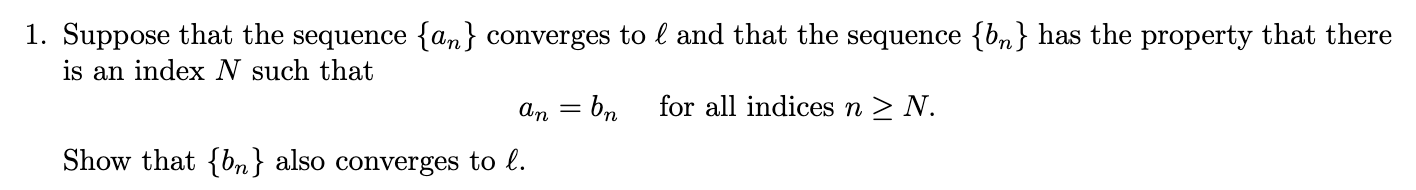
\includegraphics[width=15cm]{1.png}

\begin{proof}
  
Let us define two sequences $\{u_n\}$ and $\{v_n\}$ 
in $\RR$ with $\Lim (u_n - v_n) = 0$. We want to show then  that $\Lim (f(u_n) - f(v_n)) = 0$,
and this would satisfy the definition of uniform continuity.
Note that 
\[\{f(u_n) - f(v_n)\} = \{mu_n + b - mv_n - b\}\]
by definition of $f$. Now observe that 
\[\{mu_n + b - mv_n - b\} = \{m(u_n - v_n)\} \to m * 0 = 0\]
Therefore, $f$ is uniformly continuous on $\RR$ as desired. 

\end{proof}
\newpage 

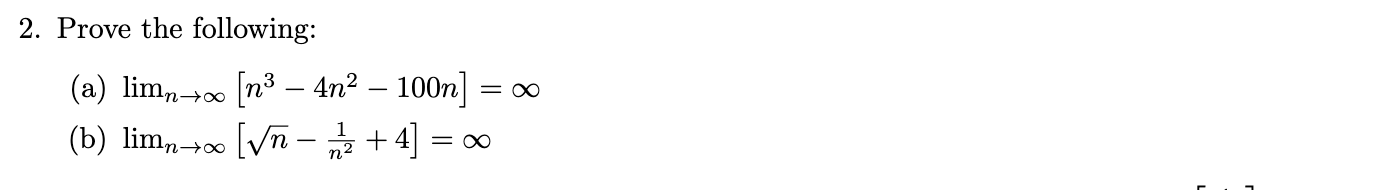
\includegraphics[width=15cm]{2.png}

\begin{proof}
  
  \hfill

\begin{enumerate}[a.]

\item We're given that $f: D \to \RR$ is uniformly continuous, and so by definition, we know 
for any two sequences $\{u_n\}, \{v_n\} \in \RR$ such that $\{u_n - v_n\} \to 0 \implies \{f(u_n) - f(v_n)\} \to 0$. 
We WTS that $\{\alpha f(u_n) - \alpha f(v_n)\} \to 0$, too. 
\[\{\alpha f(u_n) - \alpha f(v_n)\} = \{\alpha(f(u_n) - f(v_n))\} \to \alpha * 0 = 0\]
as desired, and so $\alpha f: D\to\RR$ is also uniformly continuous. 

\item Both $f, g$ are uniformly continuous so for any two sequences, $\{u_n\}, \{v_n\} \in D$ 
that converge to $0$, then their image sequences also converge to $0$. Now consider the 
function $f + g: D \to \RR$. Let us denote this new function $h$. For the same 
two sequences $\{u_n\}, \{v_n\}$ that converge to $0$, we WTS that
\[\{h(u_n) - h(v_n)\} \to 0\]
Note that 
\[\{h(u_n) - h(v_n)\} = \{f(u_n) + g(u_n) - f(v_n) - g(v_n)\}\]
by definition of $h$. 
\[= \{(f(u_n) - f(v_n)) + (g(u_n) - g(v_n))\} \to 0 + 0 = 0\]
Therefore, the function $f + g: D \to \RR$ is also uniformly continuous, as desired.

\end{enumerate}
\end{proof}
\newpage 

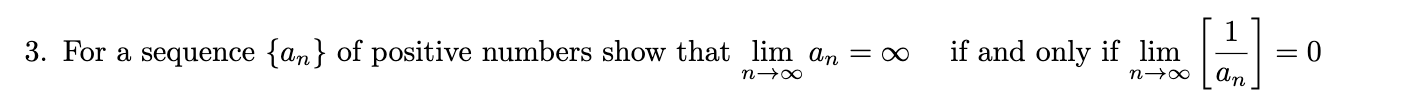
\includegraphics[width=15cm]{3.png}

\begin{proof}

To show that $f$ is not uniformly continuous, we have to find a pair of sequences
that doesn't work. Let $\{u_n\} = \{n + \frac{1}{n}\}$ and let $\{v_n\} = \{n\}$. Note 
that $\{u_n - v_n\} \to 0 $ but 
\[\{f(u_n) - f(v_n)\} = \{(n + \frac{1}{n})^3 - n^3\}\]
by definition of $f$. Note that 
\[(n + \frac{1}{n})^3 = (n + \frac{1}{n})(n^2 + 2 + \frac{1}{n^2}) = n^3 + 2n + \frac{1}{n} + n + \frac{2}{n} + \frac{1}{n^3} = n^3 + 3n + \frac{3}{n} + \frac{1}{n^3}\]
\[= \{n^3 + 3n + \frac{3}{n} + \frac{1}{n^3} - n^3\} = \{3n + \frac{3}{n} + \frac{1}{n^3}\} \to \infty \neq 0\]
by limit rules.
Therefore, $f: \RR \to \RR$ is not uniformly continuous on $\RR$. 

\end{proof}
\newpage

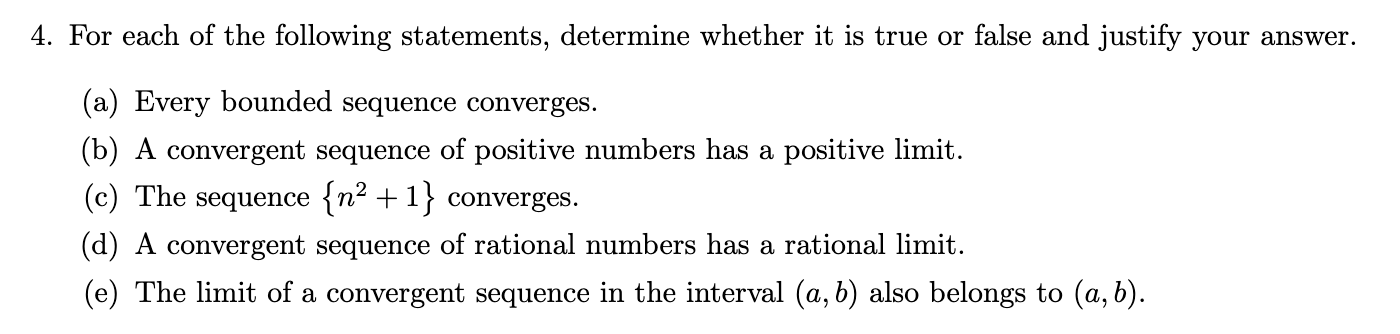
\includegraphics[width=15cm]{4.png}

\begin{proof}
  
\hfill

\begin{enumerate}[a.]

\item Let $f: D \to \RR$ be a Lipschitz function. Note that $|f(u) - f(v)| \leq C|u - v|$ for all points $u, v \in D$. 
If this works for all points in $D$, then we can construct sequences $\{u_n\}, \{v_n\} \in D$ such that the 
above still holds true for all points in the sequences. Thus, we have 
\[|f(u_n) - f(v_n)| \leq C|u_n - v_n| \ \forall \ n \ \ \ \ \ \ \ \ \ \ \ (*)\]
Recall the Comparison Lemma which states that if $\{a_n\} \to a$, then
sequence $\{b_n\} \to b$ for all $n$ greater than some threshold $N$ if $\ \exists \ c \in \RR^+$ such that 
\[|b_n - b| \leq c |a_n - a|\]
Note that we can rewrite $(*)$ as 
\[|(f(u_n) - f(v_n)) - 0| \leq C |(u_n - v_n) - 0| \ \forall \ n\]
Since we've constructed $\{u_n\}, \{v_n\} \in D$ arbitarily, we've shown that for any two sequences 
such that $\{u_n - v_n\} \to 0$ then $\{f(u_n) - f(v_n)\} \to 0$, too, and so we've shown that 
all Lipschitz functions are uniform continuous. 

\item A function $f$ satisfies $\epsilon-\delta$ criterion on $D$ if $\forall \ x_0 \in D$
then given some $\epsilon > 0, \exists \ \delta > 0$ such that 
\[\forall \ x_0 \in D, |x - x_0| < \delta \implies |f(x) - f(x_0)| < \epsilon\]
Let $\epsilon > 0$ and $\delta = \frac{\epsilon}{C}$. Observe that $\delta > 0$ because both $C, \epsilon$ are 
nonnegative. Choose any $x_0 \in D$ and let $v = x_0$. Then for all other points $x \in D$, we have that 
\[|f(x) - f(x_0)| \leq C |x - x_0|\]
by definition of the Lipschitz function.
We're given that $|x - x_0| < \delta \implies C|x-x_0| < C\delta$. Therefore, 
\[|f(x) - f(x_0)| \leq C|x-x_0| < C\delta = C * \frac{\epsilon}{C} = \epsilon\]
Therefore, $|f(x) - f(x_0)| < \epsilon$, and so Lipschitz functions satisfies the $\epsilon-\delta$ criterion on $D$. 

\end{enumerate}

\end{proof}
\newpage 

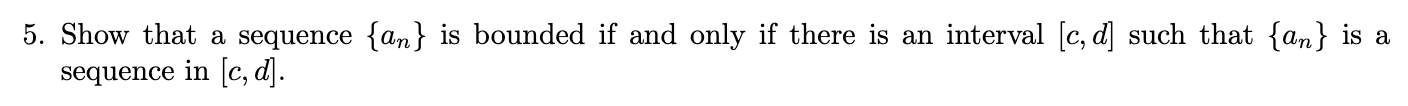
\includegraphics[width=15cm]{5.png}

\begin{proof}
  
\hfill

\begin{enumerate}[a.]

\item Let $f, g: \RR \to \RR$ and $f(x) = g(x) = x$. Note that both $f(x)$ and $g(x)$ are 
both uniformly continuous because they are linear. See problem 1 on this homework, and fix $m=1, b=0$. 
Their product, however, $h(x) = x^2$ is not uniformly continuous, as we have proved in class, 
but I will prove it again here. Consider $\{u_n\} = \{n + \frac{1}{n}\}$ and 
$\{v_n\} = \{n\}$. Note that $\{u_n - v_n\} \to 0$. However, 
\[\{h(u_n) - h(v_n)\} = \{n^2 + 2 + \frac{1}{n^2} - n^2\} \to 2 \neq 0\]
and so it is not necessarily the case that if $f: D \to \RR$ and $g: D \to \RR$ are 
both uniformly continuous, then their product is also uniformly continuous. 

\item Suppose that $f: D \to \RR$ and $g: D \to \RR$ are both uniformly continuous and bounded.
Then we know for any two sequences $\{u_n\}, \{v_n\} \in D$ that 
\[\{u_n - v_n\} \to 0 \implies \{f(u_n) - f(v_n)\} \to 0 \text{ and } \{g(u_n) - g(v_n)\} \to 0\]
Furthermore, since $f, g$ are both bounded, then $\exists \ L, M \in \RR^+$ such that 
\[|f(x)| \leq L \text{ and } |g(x)| \leq M \ \forall \ x \in D\]
Therefore, note that the product  
\[|fg(x)| \leq L * M \ \forall \ x \in D\]

Let us use the Comparison Lemma to show that $\{fg(u_n) - fg(v_n)\} \to 0$.
\[|fg(u_n) - fg(v_n)| = |f(u_n) * g(u_n) - f(v_n) * g(v_n)|\]
by the definition of product. Note that this most recent expression is bounded by 
\[\leq |L * g(u_n) + L * g(v_n)| = L|g(u_n) + g(v_n)|\]
and recall that $L > 0$ so we can pull it out of the absolute value.
\[= L|g(u_n) + g(v_n) - g(v_n) + g(v_n)| = L|g(u_n) - g(v_n) + 2g(v_n)|\]
by adding and subtracting a $g(v_n)$ from inside the absolute value.
\[\leq L|g(u_n) - g(v_n)| + 2L|g(v_n)|\] 
by the Triangle Inequality. Now by the definition of bounded,
\[\leq L|g(u_n) - g(v_n)| + 2LM\]
Note that $L, M$ are fixed in the positive real numbers. By A.P., $\exists \ c \in \RR$
such that 
\[L|g(u_n) - g(v_n)| + 2LM \leq c|g(u_n) - g(v_n)| \ \forall \ n\]
Therefore, by subtracting 0 from the first and last expressions we have 
\[|(fg(u_n) - fg(v_n)) - 0| \leq c|(g(u_n) - g(v_n)) - 0|\]
and so by the Comparison Lemma, $\{fg(u_n) - fg(v_n)\} \to 0$ and so 
$fg: D \to \RR$ is uniformly continuous as desired.
  
\end{enumerate}


\end{proof}
\newpage 

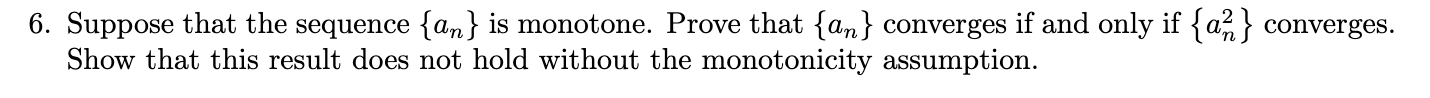
\includegraphics[width=15cm]{6.png}

\begin{proof}
  
\hfill

First, let us show the given hint. Let $x \geq 0, x_0 > 0$ then 
\[|\sqrt{x} - \sqrt{x_0}| = |\frac{x - x_0}{\sqrt{x} + \sqrt{x_0}}| \leq |\frac{x-x_0}{\sqrt{x_0}}| = \frac{1}{\sqrt{x_0}}|x - x_0|\]

\begin{enumerate}[i.]
  \item Let us show that $f(x)$ satisfies $\epsilon-\delta$ criterion at $x=4$. Let 
  $\epsilon > 0$ be given. Let $\delta = 2\epsilon$. Then if $|x - 4| < \delta$ then 
  \[|\sqrt{x} - \sqrt{4}| \leq \frac{1}{2}|x-x_0| < \frac{\delta}{2} = \epsilon\]
  \item Now let us show that $f(x)$ satisfies $\epsilon-\delta$ criterion at $x=100$. 
  Let $\epsilon > 0$ be given. Let $\delta = 10\epsilon$. Then if $|x-100| < \delta$ 
  then 
  \[|\sqrt{x} - \sqrt{100}| \leq \frac{1}{10}|x-x_0| < \frac{1}{10}\delta = \epsilon\]
\end{enumerate}

\end{proof}
\newpage 

\includegraphics[width=15cm]{7.png}


\begin{proof}
  Let $\epsilon > 0$ be given. Let $x_0 \in \RR$ and let $\delta = \frac{\epsilon}{2|x_0^2| + 3|x_0| + 1}$. Then if 
  $|x - x_0| < \delta$ then 
  \[|f(x) - f(x_0)| = |x^3 - x_0^3| = |(x-x_0) (x^2 + xx_0 + x_0^2)| < \delta |x^2 + xx_0 + x_0^2|\]
  Note that the absolute value term is a constant, but $x$ could be large, so we need to bound it.
  Let $\delta \leq 1$. Now we will examine $|x^2 + xx_0 + x_0^2|$ and try and relate it to $|x-x_0|$. 
  \[|x^2 + xx_0 + x_0^2| = |x^2 + xx_0 + x_0^2 + x_0^2 - x_0^2| = |(x^2 - x_0^2) + xx_0 + 2x_0^2|\]
  \[\leq |(x-x_0)(x + x_0)| + |xx_0| + |2x_0^2| < \delta |x + x_0| + |xx_0| + |2x_0^2|\]
  Note that it was shown in class in a similar example that $|x + x_0| < 1 + 2|x_0|$ and observe
  that the $|2x_0^2|$ is a constant already. Thus, we have 
  \[\leq \delta(1 + 2|x_0|) + |2x_0^2| + |xx_0|\]
  Now note that we have to bound $|xx_0| = |x_0||x|$ and relate it to $|x-x_0|$.
  Note that 
  \[|x| = |x - x_0 + x_0| \leq |x-x_0| + |x_0| < 1 + |x_0|\]
  Thus we get 
  \[\leq \delta ((1 + 2|x_0|) + |2x_0^2| + 1 + |x_0|) = \delta(2 + 3|x_0| + 2|x_0^2|) = \epsilon\]
  Therefore, $f(x) = x^3$ satisfies the $\epsilon-\delta$ criterion for continuity at all points 
  $x_0 \in \RR$. 
\end{proof}

\end{document}

